\chapter{PEOPLE GAZETTEER}
\label{chapter:people gazetteer}

 %Define ppl gazetteer in chapter 1 and why is it required.
People Gazetteer as defined in Chapter 1 consists of tuples of person names along with list of documents in which they occur and their corresponding topics. This chapter describes the 2-step process of construction of the People Gazetteer by
a) Extraction of person names from the news articles dataset using Named Entity Recognition in  Section~\ref{ner} and
b) Assignment of topics to news articles using LDA topic detection in  Section~\ref{topic detection}.
Output of People gazetteer developed using these steps is presented in Section ~\ref{gaz:result}.

\section{Person Named Entity Recognition (PNER)}
\label{ner}


\subsection{Definition}
NER (Named Entity Recognition) refers to classification of elements in text into pre-defined categories such as the names of persons, organizations, locations, expressions of times, quantities, monetary values, percentages, etc. 
Person Named Entity Recognition (PNER) can be defined as the process of NER that marks up only person names that occur in the text.

PNER is required in this research so as to extract all person name entities occurring in the complete dataset and identify influential person entities among them through development of the People Gazetteer. 
PNER aids in the development of People Gazetteer by first extracting all person names occurring in the dataset followed by reverse linking of a person with the articles in which he/she occurs.

\subsection{Methodology}

The Stanford CRF-NER\footnote{http://nlp.stanford.edu/software/CRF-NER.shtml} is used for PNER in this research. It can perform NER for 3 classes: Person, Organization and Location and is based on linear chain CRF (Conditional Random Field) sequence models. It is trained across several corpora and is fairly robust across multiple domains and even better when compared to some other open source NER systems as illustrated in \cite{rodriquez2012comparison}. According to their results, Stanford NER gave overall the best performance across 2 OCR datasets, and was most effective for PNER when compared with 3 other open source NER systems.


\subsection{PNER Results}

\begin{figure}[h]
  \centering
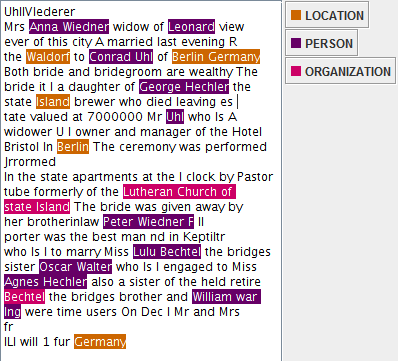
\includegraphics{NER1}
\caption{NER on a sample news article}
\label{figure:sample}
\end{figure} 




NER on a sample news article from the dataset can be seen in Figure ~\ref{figure:sample}.
 Stanford NER recognizes a person's full name as separate names by default which is rectified by combining these multi-term entities into single person entities. Person names tagged with ``PERSON" category are stored while running NER on the dataset.
Whenever a person name occurs in a document, the person entity's name along with the document name is stored to obtain tuples of person names with their document lists.
The Stanford NER takes 25 minutes to run on the complete news dataset of 14020 articles extracting a total of 38426 person entities. The output obtained can be seen in Table ~\ref{table:Table1} which shows the number of person entities with the corresponding number of documents in which they occur.  


\begin{table}[h]
  \begin{center}
\begin{tabular}{|l|l|l|}
    \hline
\textbf{No. of Person Entities} & \textbf{No. of articles} \\ \hline
36615                  & 1               \\ \hline
1122                   & 2               \\	\hline
329                    & 3               \\	\hline
123                    & 4               \\	\hline
87                     & 5               \\	\hline
48                     & 6               \\	\hline
29                     & 7               \\	\hline
19                     & 8               \\	\hline
16                     & 9               \\	\hline
5                      & 10              \\	\hline
4                      & 11              \\	\hline
6                      & 12              \\	\hline
4                      & 14              \\	\hline
3                      & 15              \\	\hline
2                      & 16              \\	\hline
1                      & 17              \\	\hline
1                      & 18              \\	\hline
3                      & 19              \\	\hline
1                      & 20              \\	\hline
1                      & 21              \\	\hline
1                      & 22              \\	\hline
1                      & 23              \\	\hline
1                      & 27              \\	\hline
1                      & 29              \\	\hline
1                      & 31              \\	\hline
1                      & 34              \\	\hline
1                      & 35              \\ 	\hline
\end{tabular}
\end{center}
\caption{Table showing output of PNER on 14020 articles}
\label{table:Table1}
\end{table}



We divide the people entities extracted into following categories so that separate analysis can be done for each category:
\begin{description}
 \item[$\bullet$Marginally Influential]: This category includes all person entities with occurrence in less than 4 news articles. (38066 person entities as calculated from Table 5.1)
\item[$\bullet$Medium Influential]: This category includes all person entities with occurrence from 4 to 15 news articles. (344 person entities) 
\item[$\bullet$Highly Influential] : This category includes all person entities with occurrence in 16 or more news articles. (16 person entities)
\end{description}



\section{Topic Detection}
\label{topic detection}

 Topic models are algorithms for discovering the main topics that occur across a large and otherwise 
unstructured collection of documents and can organize the collection according to the discovered topics.
Here, a topic refers to a set of words which describe what any document is about.
 A topic model examines the set of documents and discovers based on the statistics of the words in each, what the topics might be and what each document's balance of topics is.
Documents are considered as a mixture of topics and each topic a probability distribution over words.
 Topic detection is the process of identifying topics in a document collection using a topic model. A simple example of topic model illustrated by \cite{blei2012probabilistic} can be seen in Figure 5.2.

Topic detection is essential to this research in order to determine the topics of individual news articles that a person entity occurs in so that the person entity can be linked to the documents in which he/she occurs along with their respective topics.

\begin{figure}[h]
\begin{center}
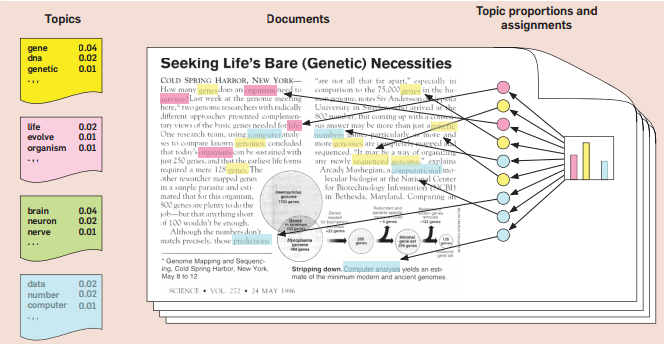
\includegraphics[scale=0.8]{topicmodel}
\caption{Simple topic modelling approach for a single article\cite{blei2012probabilistic}. Here, is being considered }
\end{center}
\end{figure} 


\subsection{Topic Detection Model}


\subsubsection{Latent Dirichlet Allocation (LDA) Model}

LDA is a generative probabilistic model in which each document is modeled as a finite mixture over an underlying set of topics and each topic, in turn, is modeled as an infinite mixture over an underlying set of topic probabilities\cite{blei2003latent}. In other words, documents exhibit multiple topics and each topic is a distribution over a fixed vocabulary.
The LDA model can be briefly reviewed as follows:


Given an input corpus of $D$ documents with $K$ topics and each topic being a multinomial distribution over a vocabulary of  $W$ words, the documents are modeled by fitting model parameters `${\Phi}$' and `${\Theta}$' . `${\Phi}$' is a matrix of size $D \times K$ in which each row is a multinomial distribution of document $d$  indicating the relative importance of words in topics. ${\Theta}$ is the matrix of size $W \times K$ with each column a multinomial distribution of topic $j$ and corresponds to the relative importance of topics in documents.

Given the observed words x = ${x_i}_j$, LDA inference is done by computing the
posterior distribution over the latent topic assignments z = ${z_i}_j$, the mixing proportions ${\Theta_j}$  and the
topics ${\Phi_k}$.  The inferencing is either done using variational bayesian methods or Gibbs sampling which involves integration and sampling of latent variables.
However, the simple LDA approach can take several days to run over a large corpora.


\subsubsection{Distributed LDA Model}
 The simple LDA method takes more time for topic modeling which is why the distributed version suits to large datasets such as ours.
The data is partitioned across separate processors and inference is done in a parallel, distributed fashion. 

The distributed LDA model as proposed by \cite{newman2009distributed} uses distributed computation where total dataset $D$ is distributed equally among multiple $P$ processors. Initialization involves data and parameters distribution to each processor and random assignment of topics so that each processor has its own copy of words $x_p$, topics $z_p$, word topic counts ${{N_w}_k}_p$ and topic counts ${{N_k}_j}_p$. 
The topic model inferencing then uses simultaneous local Gibbs sampling approach on each processor for a pre-decided number of iterations to reassign topic probabilities $z_p$, word topic ${{N_w}_k}_p$ and topic counts ${{N_k}_j}_p$.
Global update is performed after each pass by using a reduce-scatter operation on word topic count ${{N_w}_k}_p$ to get a single set of counts and obtain final topic assignments.
The model requires user set parameters before inferencing such as number of processors/threads for parallel sampling of data, number of iterations of Gibbs sampling, number of topics and Dirichlet parameters. 

\subsubsection{Topic Models Evaluation}

 Different topic models can be evaluated using the metric of ``Perplexity" which can be defined as how surprised a trained model is when given a held out test data. It has been used in \cite{newman2009distributed} and \cite{blei2003latent} for evaluating the topic detection models under different parameter settings. Perplexity can be calculated using the following formula:
$Perplexity= \exp(-\dfrac{\text{Log Likelihood of held-out test set}}{\text{No. of tokens in held-out test set}})$

 $$ \text{perplexity}(\text{test set } \boldsymbol w) = \exp \left\{ - \frac{\mathcal L(\boldsymbol w)}{\text{count of tokens}} \right\} $$

Here, held-out test set refers to the fact that complete dataset is split into two parts: one for training and the other for testing. The test set is taken as the held-out set for which perplexity is calculated. The document mixture is learned using the training data and log probability of the test data containing unseen documents is computed using the model developed.

Perplexity is a decreasing function of the log likelihood of the unseen documents as can be seen from its formula and lower the perplexity, better is the topic model.

\subsection{Results}

Parallel LDA model as described in \cite{newman2009distributed} and implemented in the Mallet\cite{McCallumMALLET} toolkit is used for topic detection over the complete dataset of 14020 news articles. 
Several topic models are first evaluated with different parameter settings in order to pre-decide the number of iterations, processors and topics for the final topic model to be used.

Perplexity is calculated by splitting the data into 90% for training and rest 10% for testing. After training with the training set with parameter settings as number of topics varying from 10 to 100, number of iterations from 100 to 500 and number of processors from 1 to 8, the log likelihood of held-out test dataset is calculated along with number of tokens in it to obtain perplexity.

\begin{figure}[h]
\begin{center}
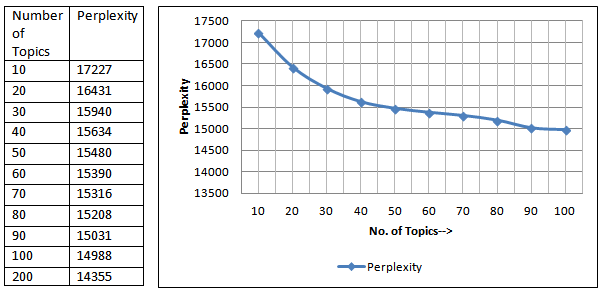
\includegraphics{topicperplex2}
\caption{Test Set Perplexity v/s Number of Topics analysis for evaluation of topic models}
\label{figure:perplex}
\end{center}
\end{figure}

Figure~\ref{figure:perplex} shows the comparison of several topic models illustrating the effect of change in number of topics on perplexity of test set. It shows decreasing perplexity with increase in number of topics along with the fact that decrease in perplexity falls with each increase in number of topics. Typically, the number of topics should be chosen as high as possible in order to consider a better model with low perplexity but the model with high number of topics also takes longer to run on a large dataset. The number of topics can also be safely chosen at the value from where further increase in number of topics does not lead to a higher decrease in perplexity. We choose number of topics as 30 (further decrease in perplexity is less from there) and 100 (lowest perplexity obtained at this value) suitable to our data to analyse their effect on the further component of influential people detection.

From the various topic models and parameter settings, the variability in perplexity with respect to the number of topics has been found to be much greater than the variability due to the number of processors or number of iterations. This is why two values of number of topics are experimented further while number of processors and number of iterations are kept fixed. The number of iterations of Gibbs sampling still need to be above the burn-in period of 200 which is why 500 is chosen as the parameter value for number of iterations. Number of threads/processors is similarly taken as 4 as least training time is obtained with this parameter value. 

The two models from topic detection are thus obtained with following parameters:
\begin{enumerate}
 \item Number of topics = 30, Number of iterations = 500, Number of threads=4 7 minutes,30 seconds
 \item Number of topics = 100, Number of iterations = 500, Number of threads=4 8 minutes 41 seconds
\end{enumerate}
The first model takes 7.5 minutes for training while the second one takes 8.6 minutes.
The set of 30 topics obtained through the first model are illustrated in Figure ~\ref{table:topicwords} and the other model with 100 topics in Appedix. 

Topic modeling gives as output, for each article in the dataset, a set of topics with their probability distribution score for the article. The topic with highest topic probability score is associated with each article in the dataset. 


\begin{table}
\resizebox{16cm}{!} {
 
   \begin{tabular}{|p{1cm}|p{16cm}|}

    \hline
    TOPIC ID & TOPIC WORDS                                                                                                                                           \\ \hline
    1        & total ii won club score night ran furlough alleys tournament time   mile fourth rolled curling scores race national game                              \\ \hline
    2        & la lu ot lo tu au tb ta ha tea day al aa ut ar uu wa tt te                                                                                            \\ \hline
    3        & iii lie tin nail tn lit hut ill ii nn thu tu anti thin inn hit lu lo   nut                                                                            \\ \hline
    4        & line street feet point western easterly northerly feel southerly   distance place distant lo fret hue beginning laid early felt                       \\ \hline
    5        & opera theatre music company week play stage evening night performance   concert mme audience manager season de orchestra house miss                   \\ \hline
    6        & great people life man women good country world american part ot ha   made la years make long place bad                                                \\ \hline
    7        & election mr party republican state district vote democratic county senator   elected city committee mayor political candidate majority york democrats \\ \hline
    8        & time ho work tn men city bo lie anti day thin long thu made part ago   lot york make                                                                  \\ \hline
    9        & st room av sun wife board front lo december rent lot november sunday   ht west ar house private si                                                    \\ \hline
    10       & dr book st story books cloth author cure free work york blood   illustrated remedy goods medical library health price                                 \\ \hline
    11       & church dr father funeral school st college sunday year rev catholic pastor services late service held society holy clock                              \\ \hline
    12       & horse race class horses won racing years prize record year show ring track mile money jockey trotting trotter ran                                     \\ \hline
    13       & cent year week pf market total net stock today central st ft lit sales short cotton ohio lot month                                                    \\ \hline
    14       & white water indian black long found thu big dog time ground wild tree killed birds bird day great lake                                                \\ \hline
    15       & price black silk goods prices ladies worth dress fine white full tea quality style wool made fancy cloth fur                                          \\ \hline
    16       & street mrs mr avenue wife house miss yesterday years home woman night ago husband found died daughter children mother                                 \\ \hline
    17       & war american government army chinese japanese china japan foreign united nov emperor states prince minister military french port navy                 \\ \hline
    18       & feet north minutes avenue boundary seconds degrees west york minute degree point east south feel city angle county laid                               \\ \hline
    19       & man ho men night back wa room left house told bad door found turned place ran lie front morning                                                       \\ \hline
    20       & water feet building boat company car train road fire miles railroad island work line city great river built bridge                                    \\ \hline
    21       & club game team play football half ball left college back yale played harvard line eleven men match yacht field                                        \\ \hline
    22       & ii iii ill lit ll si ti il im vi st iv ft mi li till lull lui oil                                                                                     \\ \hline
    23       & bank money national gold amount notes banks hank business treasury account cent paid bonds note currency company stock estate                         \\ \hline
    24       & mr john william york henry charles james club city ii george dec dr thomas smith jr brooklyn van held                                                 \\ \hline
    25       & piano st rooms car york daily chicago city sunday upright parlor furnished broadway hotel av west train brooklyn monthly                              \\ \hline
    26       & york daily steamship nov directed letter dec fur orleans al steamer walls letters close australia china japan city london                             \\ \hline
    27       & mr court police judge justice case yesterday street district witness jury charge asked attorney trial arrested lawyer told office                     \\ \hline
    28       & mr law present made public year state committee president secretary bill report states con tin united number meeting york                             \\ \hline
    29       & air ran ur fur ui full tt al tl late mr ant liar art lay told met ti tr                                                                               \\ \hline
    30       & company york trust bonds city cent railroad mortgage interest wall bond stock street st central january coupon committee jan                          \\ \hline
    \end{tabular}}
\caption{Table showing 30 topics with words and their respective ID from topic modeling}
\label{table:topicwords}
\end{table}

\newpage
\section{People Gazetteer Output }
\label{gaz:result}

The list of articles obtained for each person entity after application of PNER and highest scoring topic assigned to each article during Topic Detection are combined to obtain People Gazetteer. In each tuple of the gazetteer, a person entity gets associated with its list of articles where each article is further associated with its corresponding highest scoring topic.

A snapshot of the people gazetteer can be seen in Figure~\ref{figure:gazette} where each person entity is followed by a list consisting of a text Document ID and its corresponding Topic ID. 
\begin{figure}[!h]
\centering
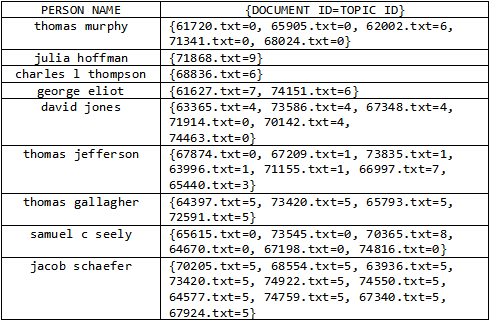
\includegraphics{gazetteer}
\caption{Snapshot of People Gazetteer with Person names, Document list of occurrence and their corresponding Topic ID}
\label{figure:gazette}
\end{figure} 

%DOUBT: Do the results of people gazetteer need to be presented separately according to each people category: marginal, medium n highly influential?
